\section{Window-Duration Sensitivity}
\label{sec:window-size-study}

\subsection{A controlled comparison on labelled traffic}

Ten minutes begins as the reference-study setting, but its suitability for
intrusion detection is assessed on the labelled Chromecast and Samsung traces.
The study compares 10-, 20-, 30-, and 60-minute non-overlapping UTC windows.
Category counts are summed within each capture. Complete observed hourly blocks
define common support at all four resolutions, preserving the same traffic and
annotated attacks. Capture-edge exclusions are recorded separately.

The normal split is fixed across durations. Where the longest duration would
have fewer than thirty calibration observations, the latest whole normal
fitting capture is reserved for calibration. Samsung therefore fits May 28--29
and calibrates May 30--31; Chromecast retains its original split. This gives
37 and 96 hourly calibration observations, respectively. The rule uses only
declared normal periods and sample counts. These study fits are distinct from
the stored reference results, whose original partitions remain unchanged.

Each duration receives a fresh normal-only DM fit and joint calibration with
the same one-percent quantile and minimum of thirty calibration observations.
The retained composition/volume/ARP detector is unchanged. Static, conservative
threshold adaptation, and conservative periodic refitting start independently
on each evaluation partition. Adaptation retains a 48-hour observed-traffic
buffer, 24-hour attempt cadence, and nominal 24 accepted hours before refitting.
Window counts scale with duration. The unchanged thirty-sample conservative
guard raises the effective refit minimum to thirty accepted hours at sixty
minutes; it is not relaxed to enable the experiment.

Original annotation hashes are checked against the saved labels. Any attack
overlap makes a window positive. Fully observed official attack intervals
provide a common detection denominator, and first-alert delay runs from attack
onset to the alerting window's close. False-alert frequency uses 24 observed
hours. A reference-grid F1 also maps each decision onto its constituent
ten-minute bins to measure temporal localisation; this does not imply an
earlier operational alert.

\subsection{Detection, false alerts, and delay}

\begin{table}[H]
\centering\small
\begin{tabular}{llrrrrr}
\toprule
\textbf{Device} & \textbf{Minutes} & \textbf{Window F1} & \textbf{Detected} &
\textbf{By end} & \textbf{FP/24 h} & \textbf{Delay (min)} \\
\midrule
Chromecast & 10 & 61.22\% & 10/18 & 9 & 0.61 & 6.83 \\
{} & 20 & 62.50\% & 9/18 & 4 & 0.30 & 13.47 \\
{} & 30 & 66.67\% & 10/18 & 3 & 0.30 & 16.99 \\
{} & 60 & 71.43\% & 11/18 & 1 & 0.00 & 36.93 \\
Samsung & 10 & 78.33\% & 28/36 & 23 & 0.78 & 5.20 \\
{} & 20 & 84.09\% & 28/36 & 13 & 0.26 & 10.38 \\
{} & 30 & 91.43\% & 35/36 & 9 & 0.52 & 17.77 \\
{} & 60 & 85.11\% & 34/36 & 5 & 1.04 & 30.93 \\
\bottomrule
\end{tabular}
\caption{Static development results on matched support. Detected attacks are
fully observed annotated intervals. ``By end'' counts alerts emitted no later
than attack end; delay is the median among detected attacks. Periodic refitting
gives the same decisions because no refit is promoted.}
\label{tab:window-duration-development}
\end{table}

\begin{figure}[H]
\centering
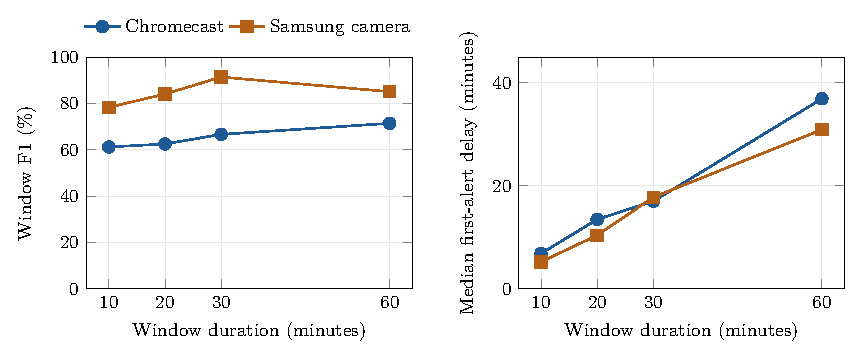
\includegraphics[width=\textwidth]{full_project_report/figures/window_size_comparison.pdf}
\caption{Static development sensitivity of window-level F1 and first-alert delay.
The saved figure uses the retained experimental CSV; lines connect the four
measured durations. Delay is conditional on detection.}
\label{fig:window-duration}
\end{figure}

Thirty minutes gives the strongest pooled static development F1: 85.11\%,
compared with 73.37\%, 78.33\%, and 81.97\% at 10, 20, and 60 minutes.
Detected attacks number 38/54, 37/54, 45/54, and 45/54, respectively. Thirty
minutes therefore improves detection coverage and reduces total false alerts
from five to three relative to ten minutes. The cost is response time: alerts
arrive by attack end for 32, 17, 12, and six attacks across the four durations.
Reference-grid localisation F1 also remains highest at ten minutes.

In the later audit, thirty-minute static detection reaches 75.00\% F1 on
Chromecast and 92.31\% on Samsung, covering all nine annotated attacks.
Hourly Chromecast reaches 100\% window F1 on only two positive windows, with
none of its three attacks alerted by attack end. Hourly Samsung F1 falls to
72.73\%, with three false alerts. Coarser labels and merged attacks change the
meaning of window-level F1. These duration-specific comparisons are separate
from the selected ten-minute final evaluation in Section~\ref{sec:final-evaluation}.

\subsection{Interaction with guarded adaptation}

Periodic refitting promotes no model and matches static detection. Threshold
adaptation changes Samsung decisions at thirty minutes and on the hourly
later sequence. Its accepted parameter changes can increase false alerts:

\begin{table}[H]
\centering\small
\begin{tabular}{llrrrr}
\toprule
\textbf{Minutes} & \textbf{Partition} & \textbf{Static F1} & \textbf{Threshold F1} &
\textbf{Static FP} & \textbf{Threshold FP} \\
\midrule
30 & Development & 91.43\% & 83.33\% & 2 & 13 \\
30 & Later audit & 92.31\% & 17.50\% & 0 & 66 \\
60 & Development & 85.11\% & 85.11\% & 4 & 4 \\
60 & Later audit & 72.73\% & 22.86\% & 3 & 27 \\
\bottomrule
\end{tabular}
\caption{Samsung threshold adaptation under the unchanged conservative policy.
Per-update movement guards do not guarantee stable future false-alert rates.}
\label{tab:window-duration-adaptation}
\end{table}

\subsection{Choice for the reference detector}

Ten minutes remains the delivered default for earlier alerts and its existing
validated starting pairs. It is not the best static coverage setting in this
sweep. Thirty minutes is a useful static candidate when longer response time
is acceptable; its gains do not transfer safely to threshold adaptation.
One hour adds delay without a consistent cross-device benefit over thirty
minutes. A production switch requires a stated response-time objective and
separate validation of the learning policy. The hourly Samsung calibration
also has limited tail resolution at 37 observations. No default configuration,
starting pair, or saved detector state is overwritten. Duration-specific
inputs, models, decisions, hashes, and complete metrics are retained.
